% Solution: Tadelis (2013) Exercise 16.8 "Beer or Quiche?". Input by \solitem.
% Rewritten and deepened from ../pratica-lecture-08-solutions/sol-tadelis-16-8.tex. Check: check_G_L07.py.
\begin{exsol}{Tadelis Exercise 16.8}{338}{Advanced}{5}
\asked (a) The extensive form of the Cho--Kreps game; (b) its BNE; (c) its PBE; (d) which PBE fail the intuitive
criterion.

\method A two-type signaling game. BNE from the type-contingent normal form; PBE by the four-step test on each
pure profile, then mixed candidates; the intuitive criterion as a restriction on off-path beliefs (Tadelis \S16.1,
pp.~319--323, and \S16.3, pp.~331--335; Gibbons \S4.4, pp.~233--244, Signaling Requirement~6). Slides: Lecture~7,
frames~38--40 (signaling games, pooling vs.\ separating), 44 (Bayes' rule), 47--48 (pooling equilibria are held up
by off-path beliefs; ``refinements (such as the intuitive criterion) rule out unreasonable beliefs''). Tadelis's
Def.~16.1 prints $v_2$ in condition~2 where the sender's payoff $v_1$ belongs (errata,
\texttt{.agent/notes/errata-game-theory-books.md}); the corrected version is used below.

\solution
\textbf{(a) Payoffs and tree.} Player~1 is a Wimp ($W$, probability $0.1$) or Surly ($S$, $0.9$). His payoff is
$1$ for his preferred breakfast ($S$: beer $B$; $W$: quiche $Q$), $0$ for the other, plus $2$ if there is no duel.
Player~2 gets $2$ from $D$ and $1$ from $N$ against $W$; $0$ from $D$ and $1$ from $N$ against $S$.
\begin{center}
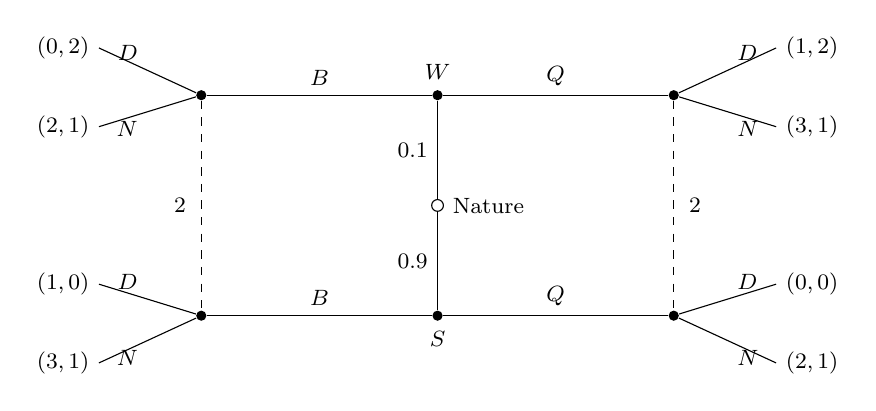
\begin{tikzpicture}[dot/.style={circle,fill,inner sep=1.3pt},every node/.style={font=\footnotesize}]
  \node[circle,draw,inner sep=1.5pt] (n) at (0,0) {};
  \node[right=2pt] at (n) {Nature};
  \node[dot,label=above:{$W$}] (w) at (0,1.4) {};
  \node[dot,label=below:{$S$}] (s) at (0,-1.4) {};
  \draw (w) -- node[left] {$0.1$} (n) -- node[left] {$0.9$} (s);
  \node[dot] (wb) at (-3,1.4) {}; \node[dot] (sb) at (-3,-1.4) {};
  \node[dot] (wq) at (3,1.4) {};  \node[dot] (sq) at (3,-1.4) {};
  \draw (w) -- node[above] {$B$} (wb);  \draw (w) -- node[above] {$Q$} (wq);
  \draw (s) -- node[above] {$B$} (sb);  \draw (s) -- node[above] {$Q$} (sq);
  \draw[dashed] (wb) -- (sb); \draw[dashed] (wq) -- (sq);
  \node[left=2pt] at (-3,0) {2}; \node[right=2pt] at (3,0) {2};
  \draw (wb) -- node[above left] {$D$} ++(-1.3,0.6) node[left] {$(0,2)$};
  \draw (wb) -- node[below left] {$N$} ++(-1.3,-0.4) node[left] {$(2,1)$};
  \draw (sb) -- node[above left] {$D$} ++(-1.3,0.4) node[left] {$(1,0)$};
  \draw (sb) -- node[below left] {$N$} ++(-1.3,-0.6) node[left] {$(3,1)$};
  \draw (wq) -- node[above right] {$D$} ++(1.3,0.6) node[right] {$(1,2)$};
  \draw (wq) -- node[below right] {$N$} ++(1.3,-0.4) node[right] {$(3,1)$};
  \draw (sq) -- node[above right] {$D$} ++(1.3,0.4) node[right] {$(0,0)$};
  \draw (sq) -- node[below right] {$N$} ++(1.3,-0.6) node[right] {$(2,1)$};
\end{tikzpicture}
\end{center}
\textbf{Player~2's best reply.} With $\mu = \Pr(W \mid \text{breakfast})$: $D$ gives $2\mu$, $N$ gives $1$. He duels
iff $\mu \ge \frac12$. The prior, $0.1$, is far below $\frac12$.

\textbf{A key identity.} Let $d_B, d_Q$ be the probabilities of a duel after $B$ and after $Q$. Then
\[
  u_S(B) - u_S(Q) = 1 - 2d_B + 2d_Q, \qquad u_W(B) - u_W(Q) = -1 - 2d_B + 2d_Q :
\]
whatever player~2 does, Surly gains exactly $2$ more from beer than Wimp does.

\textbf{(c) PBE (pure profiles first).} Profiles are (breakfast of $W$, breakfast of $S$).
\begin{itemize}
  \item \emph{Separating $(Q, B)$.} Bayes: $\mu(Q) = 1$, so $D$ after $Q$; $\mu(B) = 0$, so $N$ after $B$. $W$ gets
  $1$ from quiche but $2$ from beer: deviates. Not a PBE.
  \item \emph{Reverse $(B, Q)$.} $D$ after $B$, $N$ after $Q$: $W$ gets $0$ but $3$ from quiche. Not a PBE.
  \item \emph{Pooling on beer $(B, B)$.} Bayes: $\mu(B) = 0.1$, so $N$ after $B$. $S$ gets $3$, the best possible.
  $W$ gets $2$, and $3 - 2d_Q$ from quiche, so he stays iff $d_Q \ge \frac12$, which needs
  $\mu(Q) \ge \frac12$ ($\mu(Q) > \frac12$ for a sure duel). \textbf{PBE}: both drink beer; $N$ after $B$; $D$
  after $Q$; off-path belief $\Pr(W \mid Q) \ge \frac12$.
  \item \emph{Pooling on quiche $(Q, Q)$.} $\mu(Q) = 0.1$, so $N$ after $Q$. $W$ gets $3$. $S$ gets $2$, and
  $3 - 2d_B$ from beer, so he stays iff $d_B \ge \frac12$, which needs $\Pr(W \mid B) \ge \frac12$. \textbf{PBE}:
  both eat quiche; $N$ after $Q$; $D$ after $B$; off-path belief $\Pr(W \mid B) \ge \frac12$.
\end{itemize}
\emph{No mixed (semi-separating) PBE.} If $W$ is willing to mix, he is indifferent, and by the identity Surly then
strictly prefers beer; so beer comes from both types with $\mu(B) \le 0.1$ ($N$ after $B$) and quiche from $W$
only ($\mu(Q) = 1$, $D$ after $Q$). Then $W$ gets $2$ from beer and $1$ from quiche: not indifferent.
If $W$ plays $Q$ for sure and $S$ mixes, then $\mu(B) = 0$, $N$ after $B$, and Surly strictly prefers beer
($3 > 2$): he does not mix. So the PBE are the two pooling families.

\textbf{(b) BNE.} The two pooling profiles above, with player~2's reply to the unused breakfast being $D$ (a
duel with probability at least $\frac12$ if mixed). Separating profiles fail for the same reasons as in (c), since
both of player~2's information sets are reached there. Here every pure BNE is also a PBE: the off-path reply
$D$ is supported by a belief $\mu \ge \frac12$.

\textbf{(d) Intuitive criterion} (corrected Def.~16.1). In a PBE with payoffs $v_1^*(t)$, a message $m$ is
\emph{equilibrium-dominated} for type $t$ if $v_1^*(t) > \max_a u_1(t, m, a)$. After an off-path $m$, player~2
must put zero weight on types for which $m$ is equilibrium-dominated (if some type remains). The PBE fails if,
under the restricted beliefs, some type gains by deviating to $m$.
\begin{itemize}
  \item \emph{Pooling on quiche fails.} Equilibrium payoffs: $W$ $3$, $S$ $2$. Beer gives $W$ at most $2 < 3$:
  equilibrium-dominated for $W$. It gives $S$ up to $3 > 2$: not dominated. So after beer player~2 must believe
  Surly ($\mu(B) = 0$) and not duel, and then $S$ gains by deviating to beer ($3 > 2$).
  \item \emph{Pooling on beer survives.} Equilibrium payoffs: $W$ $2$, $S$ $3$. Quiche gives $S$ at most $2 < 3$:
  dominated for $S$. It gives $W$ up to $3 > 2$: not dominated. So after quiche player~2 must believe Wimp
  ($\mu(Q) = 1$) and duel; $W$ then gets $1 < 2$ from quiche. No type gains: the belief the equilibrium needed
  is exactly the one the criterion allows.
\end{itemize}

\interp The criterion reads a deviation as a speech: ``I would not eat beer if I were the wimp, since that cannot
beat what I am getting; so if you see me drinking beer, conclude I am surly.'' Pooling on quiche needs player~2 to
believe the opposite, which is the kind of unreasonable off-path belief frame~48 warns about. The game also shows
that PBE alone does not pin down the outcome: two pooling equilibria with opposite breakfasts both pass
Requirements~1--4.

\verify \texttt{check\_G\_L07.py} builds the game from the story, enumerates pure profiles (the BNE and the PBE are
exactly the two pooling profiles, with off-path beliefs $\Pr(W \mid \cdot) \in [\frac12, 1]$), checks the identity
symbolically (Surly gains $2$ more; when $W$ is indifferent Surly strictly prefers beer) and applies the
equilibrium-dominance test to both. Output: ``Tadelis 16.8: BNE = PBE = pooling on beer (D after Q, Pr(W|Q) >= 1/2)
and on quiche (D after B, Pr(W|B) >= 1/2); no separating; quiche fails the intuitive criterion''. Tadelis prints no
answer.

\mistakes
\begin{itemize}
  \item Running the intuitive criterion backwards: removing the type for which the deviation \emph{could} pay.
  One removes the type for which it can \emph{never} pay (beer is dominated for the wimp in the quiche equilibrium).
  \item Using player~2's payoffs in the domination test, as Tadelis's misprinted Def.~16.1 suggests. Equilibrium
  dominance compares the \emph{sender's} payoffs.
  \item Setting $\mu(B) = 0.1$ after beer in the quiche equilibrium ``by Bayes' rule''. Beer is off the path; the
  prior is not the off-path belief.
  \item Expecting a separating equilibrium because the types have different tastes. The duel threat (worth $2$)
  outweighs the breakfast (worth $1$), so the wimp always imitates when that avoids a duel.
  \item Concluding that BNE and PBE coincide in general. They coincide here only because the off-path duel can
  be justified by some belief.
\end{itemize}

\answer{(b) BNE: pooling on beer ($N$ after beer, $D$ after quiche) and pooling on quiche ($N$ after quiche, $D$
after beer). (c) The same two are the PBE, with off-path beliefs $\Pr(W \mid Q) \ge \frac12$ and
$\Pr(W \mid B) \ge \frac12$ respectively; there is no separating or semi-separating PBE. (d) Pooling on quiche fails
the intuitive criterion (beer is equilibrium-dominated for the wimp, so a beer drinker must be surly, who then
deviates); pooling on beer survives.}
\end{exsol}
